\subsection{Анализ архитектурных подходов и~технологий для~построения iOS-клиента}
\label{sec:analysis:research:mobArch}

Любое современное мобильное программное средство отображает динамически изменяемое содержимое, часто изменение одного поля модели способно повлечь за собой массу изменений в~пользовательском интерфейсе. Важной проблемой при~проектировании архитектуры мобильного программного средства является консистентность состояния, данных и~пользовательского интерфейса. Последние несколько лет сфера пытается уйти от~императивного стиля программирования в~сторону декларативного, для~этого было разработано множество подходов, архитектур и~инструментов. Одним из~подходов является реактивное программирование и~его конкретная имплементация -- \gls{rx}. Ниже будут рассмотрены традиционные подходы и~инструменты, используемые при~проектировании и~имплементации архитектуры мобильного iOS клиента.

\subsubsection {}
\label{sec:analysis:research:mobArch:mvc}

Классическим архитектурным паттером при разработке для платформы iOS является \gls{mvc}. Шаблон присваивает объектам в приложении одну из трех ролей: модель, представление или контроллер. Шаблон определяет не только роли объектов в приложении, но и способ взаимодействия объектов друг с другом. Каждый из трех типов объектов отделен от других абстрактными границами и связывается с объектами других типов через эти границы. Набор объектов определенного типа \gls{mvc} в приложении иногда называется слоем, например, слоем модели\cite{apple:mvc}. На рисунке \ref{sec:analysis:research:mobArch:apple-mvc:image:mvc} представлена связь между объектами паттерна \gls{mvc}.

\begin{figure}[h]
  \centering
    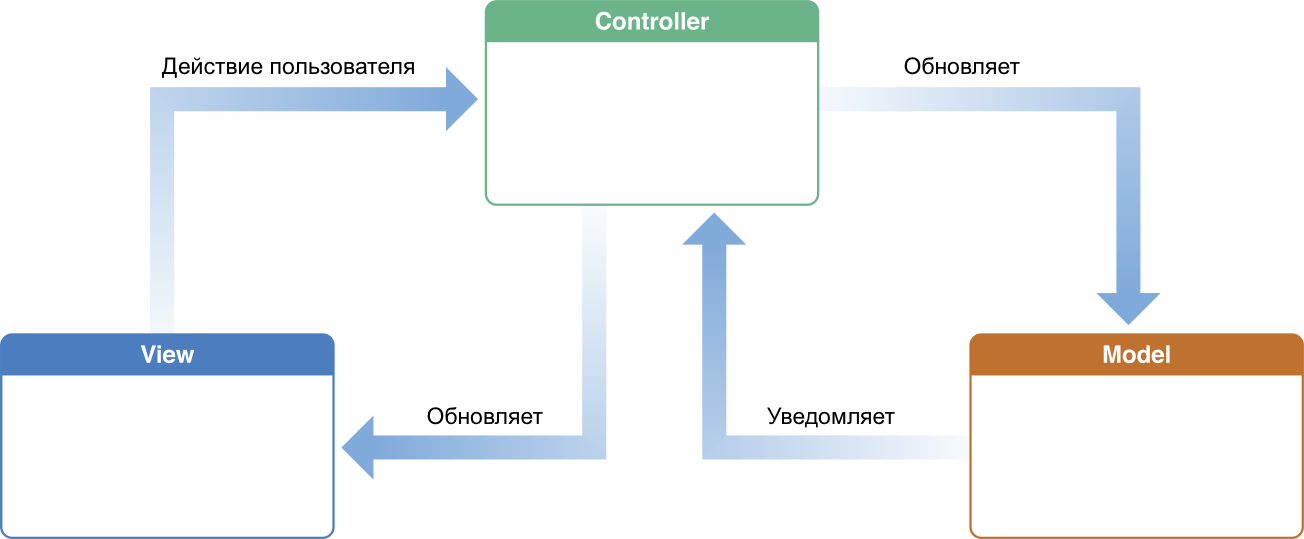
\includegraphics[width=1\textwidth]{inc/img/mvc.png}
  \caption{Связи между объектами MVC}
  \label{sec:analysis:research:mobArch:apple-mvc:image:mvc}
\end{figure}

\emph{Объекты модели} инкапсулируют данные, специфические для приложения и описывают логику изменения этих данных. Для примера, объект модели может представлять персонажа в игре или контакт в книге контактов. Объекты модели могут иметь связь один ко многим или многие ко многим с остальными объектами модели, и поэтому иногда модельный уровень приложения представляет собой один или более объектных графов. В хорошей реализации паттерна объекты модели не должны иметь связи с объектами представления, изолируя данные от ошибок слоя презентации и действий пользователя: пользовательские действия в слое презентации, которые создают или модифицируют данные, влияют на модель при помощи промежуточного слоя котроллер и являются причиной создания или обновления объектов модели. Когда объект модели изменяется (например, новые данные были получены из сети), он уведомляет объект контроллера, который, в свою очередь, обновляет объект представления.

\emph{Объектами представления} являются объекты, которые видит пользователь. Объекты данной группы умеют представлять себя графически на экране и реагировать на действия пользователя. Основной задачей объектов представления является вывести данные из модели приложения и позволить пользователю редактировать эти данные. Объекты представления часто обобщатся и используются между приложениями, хорошим примером такого переиспользования является \gls{uikit}. 

Объекты типа \emph{котроллер} являются прослойкой между моделью и представлением, уведомляющих представление об изменениях в модели и наоборот. Объекты контроллера также могут выполнять настройку и координирование задач для приложения и управлять жизненными циклами других объектов. 
\subsubsection {}
\label{sec:analysis:research:mobArch:mvvm}

Шаблон \gls{mvvm} применяется при проектировании архитектуры приложения и позволяет разделить модель, представление и логику её представления. Первоначально был представлен сообществу Джоном Госсманом (John Gossman) в 2005 году как модификация шаблона Presentation Model\cite{wiki:mvvm}.

\gls{mvvm} является альтернативой паттерну \gls{mvc}. С паттерном \gls{mvvm} тесно связан паттерн <<связывание данных>>, позволяющий задать двухстороннюю связь между данными и отображением (сильно упрощая решение задачи динамически обновляемого контента). Шаблон состоит из трёх частей, связанных определённым образом: Model, View, ViewModel.

\emph{Model} (Модель) представляет собой бизнес логику и фундаментальные данные, необходимые для работы приложения.

\emph{View} (Представление) -- графический интерфейс, то есть окно, кнопки и так продолжая. Представление является подписчиком на события изменений значений свойств и пользователем команд, предоставляемых Моделью Представления.

\emph{ViewModel} (Модель Представления) является прослойкой между Моделью и Представлением, предоставляя подготовленные для связывания данные из Модели и набор команд для изменения Модели Представлением.

Шаблон отвечает всем поставленным требованиям: является лёгким в использовании, позволяет разделить интерфейс на независимые компоненты, которые в будущем могут быть доработаны без необходимости дополнительных изменений в Представлении и имеет паттерны для динамического обновления данных\cite{app-architecture}. Исходя из этого было принято решение выбрать \gls{mvvm} в качестве основы для будущей архитектуры пользовательского интерфейса приложения.
\subsubsection{}
\label{sec:analysis:research:mobArch:ufeature}

По своей сути приложения состоят из набора функциональных возможностей. Обычно все возможности приложения реализованы в пределах одного модуля. Результатом такого подхода является тесная связанность разных модулей, введение неявных зависимостей, увеличение сложности поддержки и разработки новых функций. Паттерн \gls{mvvm} предназначен для организации пользовательского интерфейса приложения, однако часто приложение можно условно разбить на несколько независимых доменов -- обычно каждый такой домен называется микросервисом.

Микросервисы предоставляют минимальный, но необходимый для интеграции \gls{api}, скрывая детали реализации. Для примера в iOS клиенте чата можно выделить следующие домены:

\begin{itemize}
	\item сервисы для шифрования сообщений, общения с сервером, работой с базой;
	\item экраны списка контактов, настроек, списка диалогов и конкретного диалога.
\end{itemize}

В 2016 году компания SoundCloud представила своё видение организации микросервисной архитектуры в мобильных приложениях: \glspl{ufeature}.

\glspl{ufeature} -- архитектурный подход для стуктурирования iOS приложений, предоставляющий масштабируемость, оптимизацию времени сборки проетка и циклов тестирования, гарантирующий адоптацию хороших практик разработки в команде. Основной идеей подхода является разработка независимых возможностей приложения, которые взаимодействуют при помощи чётко обозначенного \gls{api}\cite{soundcloud:ufeature}.

Типичная \gls{ufeature} представляет из себя отдельный проект с 4 схемами:

\begin{itemize}
	\item код и ресурсы;
	\item тесты;
	\item данные, которые используются в тестах и приложении-примере;
	\item приложение-пример.
\end{itemize}

На рисунке \ref{sec:analysis:research:mobArch:ufeature:featureDependencyDiagram} представлена связь схем одного модуля \gls{ufeature}.

\begin{figure}[h]
  \centering
    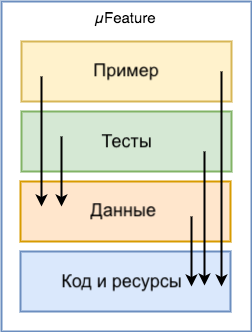
\includegraphics{inc/img/ufeature-diagram.png}
  \caption{Организация схем внутри модуля одной uFeature}
  \label{sec:analysis:research:mobArch:ufeature:featureDependencyDiagram}
\end{figure}

Автор подхода предлагает разделять все \gls{ufeature} на два вида:

\begin{itemize}
	\item \emph{Foundation} -- основные строительные блоки, общие расширение пользовательского интерфейса, сервисы;
	\item \emph{Product} -- возможности, с которыми пользователь взаимодействует и видит на экране, например список диалогов;
\end{itemize}


\subsubsection{}
\label{sec:analysis:research:mobArch:fp}

\emph{Функциональное программирование} --- раздел дискретной математики и парадигма программирования, в которой процесс выполнения трактуется как вычисление значений функций в математическом понимании последних (в отличие от функций как подпрограмм в процедурном программировании). Функциональное программирование предполагает обходиться вычислением результатов функций от исходных данных и результатов других функций, и не предполагает явного хранения состояния программы. Соответственно, не предполагает оно и изменяемость этого состояния. \cite{wiki:fp}

После прочтения определения функционального программирования становится очевидно, что использовать исключительно этот подход при построении интерактивного приложения с пользовательским интерфейсом является крайне сложной задачей. В приложениях данного типа состояние навязывается и требованиями и операционной системой. Тем не менее существует ряд функциональных подходов, соблюдение которых значительно понижает количество ошибок:

\begin{itemize}
\item отсутствие глобального состояния;
\item отсутствие изменяемого состояния;
\item чистые функции;
\item функции высших порядков;
\item рекурсия.
\end{itemize}

После обобщения и ослабления некоторых признаков, были выведены следующие принципы будущей архитектуры:

\begin{enumerate}
\item \emph{Сокращение глобального состояния}. Данный пункт не подразумевает полный отказ от глобального состояния, однако призывает как можно больше данных передавать при инициализации, параметрами методов или в виде \gls{observable}.
\item \emph{Модульность}. Концепция чистой функции позволяет трактовать программу, как результат применения цепочки функций, следовательно всё приложение(и его отдельные части) можно декомпозировать на множество чистых функций, что позволяет повысить тестируемость и побуждает избегать неявных зависимостей.
\item \emph {Аккуратное использование изменяемого состояния}. Данный принцип призывает делать выбор в пользу неизменяемых типов данных, передаваемых по значению. 
\item \emph {Ответственный дизайн типов}. Функциональная программа с хорошим дизайном крайне трепетно относится к используемым типам, описывая ими все возможные побочные эффекты и структурируя код. Огромное количество ошибок разработчика обнаруживается на стадии компиляции.
\end{enumerate}

К сожалению, компилятор языка Swift не гарантирует оптимизацию хвостовой рекурсии, поэтому от идеи повсеместного использования рекурсии было решено отказаться в пользу богатого набора функций высшего порядка в стандартной библиотеке. В пункте \ref{sec:development:arch:ios:swift} будут раскрыты особенности языка Swift, которые помогают эффективно использовать описанные выше принципы, такие как \gls{cow}, функции высшего порядка, замыкания, Optional и некоторые другие.
\subsubsection{}
\label{sec:analysis:research:mobArch:dataflow}

\textbf{Data flow} -- подход к~программированию, при~котором программа моделируется в~виде ориентированного графа потока данных между операциями\cite{wiki:data-flow}.

Традиционно программа моделируется как последовательность операций, происходящих в~определённом порядке. Программирование потоков данных подчёркивает перемещение данных и~рассматривает программное средство как последовательность переходов. Явно определённые входы и~выходы соединяют операции. Программы данного типа часто представлены в~виде набора текстовых инструкций, которые описывают систему, последовательно передающую данные между небольшими инструментами, которые получают данные, модифицируют их и~возвращают результат. 

\subsubsection{}
\label{sec:analysis:research:mobArch:reactive}

Реактивное программирование представляет собой асинхронную парадигму программирования, связанную с~программированием потоков данных и~распространением изменений. Языки с~поддержкой парадигмы реактивного программирования позволяют описать статические и~динамические потоки данных, имеют механизмы для~уведомления подписчиков об изменениях. Например, выполнение операции \(a = c + b\) запишет в~переменную \(a\) значение суммы \(b + c\). Последующее изменение \(b\) или~\(c\) никак не отразится на~переменной \(a\). В~реактивном же программировании \(a\) будет обновлено при~изменении любой переменной, которая участвует при~вычислении значения \(a\).
Удобно выделять три типа программ:
\begin{enumerate}
	\item \emph{Программы трансформации} вычисляют результат для~полученного набора входящих данных, типичным примером является компилятор или~программы для~расчётов;
	\item \emph{Интерактивные программы} взаимодействуют с~собственной скоростью с~пользователем или~другой программой;
	\item \emph{Реактивные программы} также поддерживают непрерывное взаимодействие с~окружением, однако со скоростью, диктуемой этим окружением.
\end{enumerate}
Интерактивные программы работают в~собственном темпе, когда реактивные могут работать только в~ответ на~внешние требования.
\subsubsection{}
\label{sec:analysis:research:mobArch:rx}

\emph{Reactive Extensions} -- набор средств и \gls{api}, позволяющие императивным языкам программирования использовать концепции реактивного программирования и потоки данных независимо от того, являются ли потоки синхронными или асинхронными\cite{wiki:rx}.

\gls{rx} объединяет лучшие идеи паттерна \gls{observer}, Iterable и функционального программировния. Парадигма дополняет паттерн \gls{observer}, добавляет набор операторов для декларативного описания трансформации и композиции потоков, абстрагируя вопросы синхронизации, потокобезопасности.

Одной из важнейших гарантий \gls{rx} является порядок, в котором подписчик получит данные. \gls{observer} обрабатывает каждое событие по порядку, не более одного за раз, если события успевают поступать быстрее, чем подписчик их потребляет -- события ставятся в очередь или откидываются.

Основным примитивом \gls{rx} является \emph{\gls{observable}}. Observable является идеальным способом рассылки асинхронных событий.

\begin{table}[h!]
\caption{Разные способы получения значений}
\label{theory:archeticture:rx:call}
\centering
\begin{tabularx}{\textwidth}{ |X|X|X| } 
 \hline
  & \emph{Одно значение} & \emph{Несколько значений} \\ 
 \hline
 \emph{Синхронно} & T getData() & Iterable<T> getData() \\ 
 \hline
 \emph{Асинхронно} & Future<T> & Observable<T> getData() \\ 
 \hline
\end{tabularx}
\end{table}

Создатели \gls{rx} предлагают\cite{reactivex:introduction} рассматривать \gls{observable} как эквивалент Iterable с моделью push (данные приходят, а не запрашиваются потребителем). В таблице \ref{theory:archeticture:rx:iterable-observable} рассмотрены аналогичные возможности Iterable и \gls{observable}

\begin{table}[h!]
\caption{Сравнение Observable и Iterable}
\label{theory:archeticture:rx:iterable-observable}
\centering
\begin{tabularx}{\textwidth}{ |X|X|X| } 
 \hline
 \emph{Событие} & \emph{Iterable(pull)} & \emph{Obsevable(push)} \\ 
 \hline
 \emph{Получение данных} & T next() & onNext(T) \\ 
 \hline
 \emph{Ошибка} & throw & onError(Error) \\ 
 \hline
  \emph{Завершение} & !hasNext() & onCompleted() \\ 
 \hline
\end{tabularx}
\end{table}

\gls{observable} принято разделять на \emph{холодные} и \emph{горячие}. Различие заключается в том, когда \gls{observable} начинает высылать значения, когда выполняется логика подписки. Холодный \gls{observable} запускает работу при каждой подписке, следовательно высылает полный набор значений каждому подписчику. Горячий \gls{observable} начинает работу (и рассылку событий) при создании, подписчики получают только события, которые были высланы после подписки, у горячих \gls{observable} нет возможности запустить работу заново. Хорошим примером отличия горячих и холодных \gls{observable} является сетевой запрос:

\begin{enumerate}
	\item Холодный \gls{observable} будет выполнять запрос при каждой новой подписке, высылая результат каждому новому подписчику.
	\item Горячий \gls{observable} отправит запрос при создании, результат получат только те подписчики, которые сформировали подписку до получения ответа от сети.
\end{enumerate}

Существуют способы охладить или подогреть \gls{observable}, заставить горячий \gls{observable} высылать определённое количество последних событий всем новым подписчикам, отложить его работу до вызова метода connect.

\gls{observable} и \gls{observer} являются важными компонентами \gls{rx}, но не единственными. Сами по себе они не делают ничего, кроме небольшого расширения привычного паттерна \gls{observer}, адаптированного для работы с последовательностью событий. Настоящая сила \gls{rx} приходит с так называемыми реактивными расширениями: операторами, которые позволяют трансформировать, комбинировать и манипулировать значениями, произведёнными \gls{observable}. Эти расширения позволяют декларативно компоновать асинхронные последовательности с высокой производительностью колбеков, но без побочных эффектов в виде высокой вложенности и кода-лапши.

\emph{Оператор} -- функция, которая принимает \gls{observable} своим первым аргументом и возвращает другой \gls{observable}, который является результатом некоторой трансформации элементов из первого \gls{observable}.

Таким образом, были рассмотрены основные архитектурные подходы и~парадигмы в~современной разработке мобильных программных средства.